\section{Case 1}
For case 1 the linear multiple measurement vector model
\begin{align*}
Y = AX,
\end{align*}
with $Y \in \mathbb{R}^{m \times L}$ being a known measurement matrix, $A \in \mathbb{R}^{m \times n}$ a known mixing matrix and $X \in \mathbb{R}^{n \times L}$ being the source matrix we wish to recover in this case.
\\
The known matrices $Y$ and $A$ has been generated from a \texttt{sklearn}-package in Python. The commando used from this package is the \texttt{make\_sparse\_coded\_signal} with the inputs \texttt{(n\_samples = L, n\_components = n, n\_features = m, n\_nonzero\_coefs = k)}. The function generate a signal as a sparse combination of dictionary elements.
\\
The source matrix wish recovered $X$ is also generated from this function and will be used to be compared with the recovered/estimated source matrix $X_{cal}$. $X_{cal}$ will be recovered with the M-SBL Algorithm with the following variables: 
\begin{itemize}
\item $m = 30$ (number of sensors)
\item $n = 80$ (number of sources)
\item $L = 20$ (number of samples)
\item No segmentations -- $Y = AX$
\item Iterations = 1000
\item $k = 40$ is active sources (row-wise) and is half of the rows in $X$ ($k$ is the non-zeros rows.)   
\end{itemize}
For the comparison we start with visualising the second row of $X$ and $X_{cal}$ which is one source ($N=1$) with $L = 20$ samples and the second column of $X$ and $X_{cal}$ which one sample $L=1$ with $N = 80$ sources.
\begin{figure}[H]
\centering
\begin{subfigure}{0.49\textwidth}
\centering
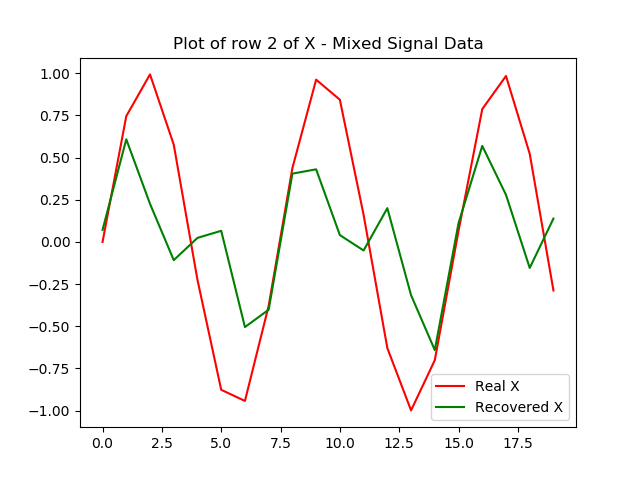
\includegraphics[width=\textwidth]{figures/cases/case1_1.png}
\caption{}
\label{fig:case1_1}
\end{subfigure}
\begin{subfigure}{0.49\textwidth}
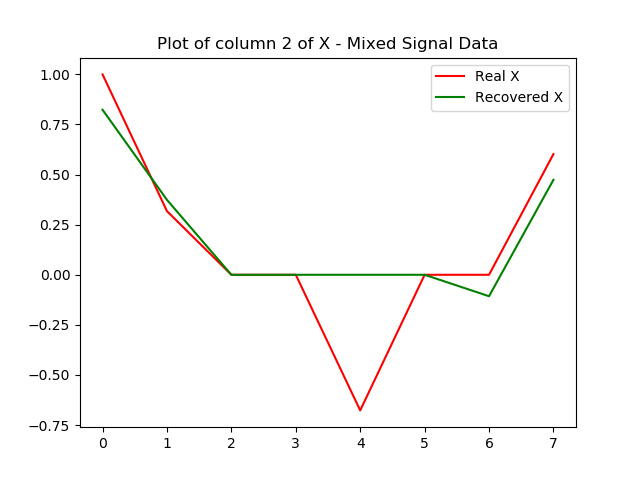
\includegraphics[width=\textwidth]{figures/cases/case1_2.png}
\caption{}
\label{fig:case1_2}
\end{subfigure}
\caption{\textbf{(a)} The comparison of one source of all the samples of the real $X$ and the recovered $X_{cal}$. \textbf{(b)} The comparison of one samples for all sources of the real $X$ and the recovered $X_{cal}$.}
\end{figure}
\noindent
We have found the error between all the elements of the known/real $X$ and the recovered/estimated $X_{cal}$ by using the mean square error (MSE) and it was found to be $0.38$ rounded to the first 2 decimals.
\\ \\
By looking at the elements in both source matrices it was found the that function we use to create the known $X$ is not row sparse meaning that some elements in the rows are non-zeros leading all the source to be active. This differ from our recovered $X_{cal}$ which is row sparse as it have $n - k$ zero rows. This can also be seen when we visualise the first four sources in $X$ and $X_{cal}$.
\begin{figure}[H]
\centering
\begin{subfigure}{0.49\textwidth}
\centering
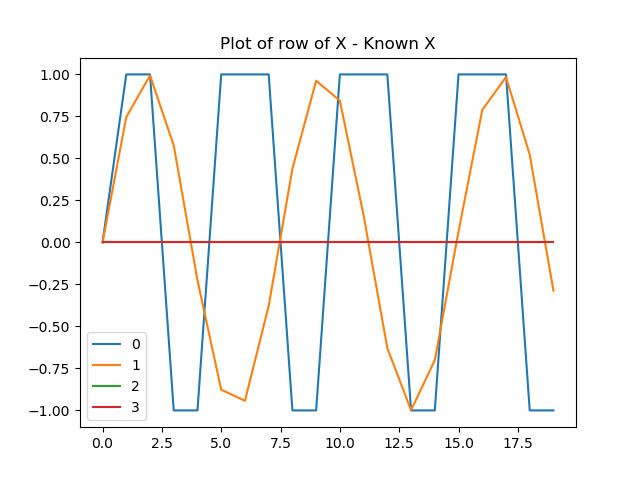
\includegraphics[width=\textwidth]{figures/cases/case1_3.png}
\caption{}
\label{fig:case1_3}
\end{subfigure}
\begin{subfigure}{0.49\textwidth}
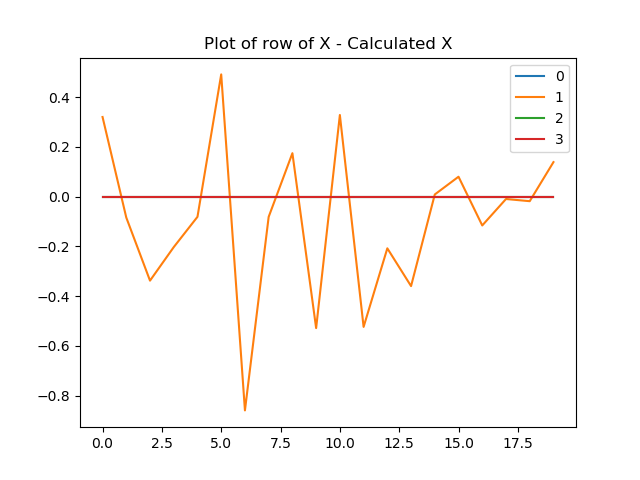
\includegraphics[width=\textwidth]{figures/cases/case1_4.png}
\caption{}
\label{fig:case1_4}
\end{subfigure}
\caption{\textbf{(a)} The first four sources of $X$ \textbf{(b)} The first four sources of $X_{cal}$. Only source $1$ is active.}
\end{figure}
\noindent